%!TEX TS-program = ../make.zsh

\begin{frame}{Resources}
  \begin{center}
    \textbf{Scripts and plots for this talk}: \\ \vspace{0.2cm}
    \url{https://github.com/fiedl/hole-ice-study/issues/117}

    \vspace{1cm}

    \textbf{YouTube video with Steamshovel vizualition}: \\ \vspace{0.2cm}
    \url{https://www.youtube.com/watch?v=M_QGNdGG9Ew}

    \vspace{1cm}

    Thesis (2018-09-05) with more info on direct hole-ice simulation: \\ \vspace{0.2cm}
    \url{https://github.com/fiedl/hole-ice-latex}

    \vspace{1cm}

    Previous talks: \\ \vspace{0.2cm}
    \url{https://github.com/fiedl/hole-ice-talk/releases}

    \vspace{1cm}

    \LaTeX\ version of these presentation slides: \\ \vspace{0.2cm}
    \url{https://github.com/fiedl/hole-ice-talk}
  \end{center}
\end{frame}

\section{Simulation scenario}
\begin{frame}[fragile]{Simulation scenario}
  For each angle polar and azimuthal angle, shoot photons onto the DOM, possibly propagate through the bubble column, and count hits.

  \begin{columns}
    \begin{column}{0.5\textwidth}
      \begin{figure}
        \includegraphics[width=0.9\textwidth]{img/angular-acceptance-coordinates-plane-waves-Ii2nieki}
        \caption{View from the side. Shooting photons from different polar angles.}
      \end{figure}
    \end{column}
    \begin{column}{0.5\textwidth}
      \begin{figure}
        \includegraphics[width=0.9\textwidth]{img/summerscenario-003}
        \caption{View from above. Shooting photons from different azimuthal angles.}
      \end{figure}
    \end{column}
  \end{columns}
\end{frame}

\section{Simulation results}
\subsection{bubble-column radius $7.5\cm$, geometric scattering length $10\cm$}
\begin{frame}[fragile]{Simulation results}
  \begin{columns}
    \begin{column}{0.5\textwidth}
      \includegraphics[width=\textwidth]{img/summer_scenario_r7-5cm_sca10cm}
    \end{column}
    \begin{column}{0.5\textwidth}
      \includegraphics[width=0.8\textwidth]{img/summerscenario-003}
    \end{column}
  \end{columns}

  \tiny Total photon hit count: 12968 / 1e6

  \tiny Configuration: Starting distance $3\m$, plane-wave extent $3\m$, bubble-column geometric scattering length $10\cm$, bulk-ice geometric scattering length $130\cm$.
  \normalsize

  \begin{itemize}
    \item For lower polar angles ($\cos\eta \approx 1$), less photons should arrive from azimuths B and C as from azimuth A
      \tiny as the DOM's PMTs look downwards and photons from B and C are more likely to cross the bubble-column cylinder. \normalsize
    \item From azimuths B and C, the same number of photons should arrive \tiny due to the symmetry of the scenario (right image). \normalsize
  \end{itemize}
\end{frame}

\subsection{bubble-column radius $15\cm$, geometric scattering length $10\cm$}
\begin{frame}[fragile]{Simulation results}
  \begin{columns}
    \begin{column}{0.5\textwidth}
      \includegraphics[width=\textwidth]{img/summer_scenario_r15cm_sca10cm}
    \end{column}
    \begin{column}{0.5\textwidth}
      \includegraphics[width=0.8\textwidth]{img/summerscenario-004}
    \end{column}
  \end{columns}

  \tiny Total photon hit count: 11600 / 1e6

  \tiny Configuration: Starting distance $3\m$, plane-wave extent $3\m$, bubble-column geometric scattering length $10\cm$, bulk-ice geometric scattering length $130\cm$.
  \normalsize

  \begin{itemize}
    \item For a larger bubble column with same scattering lenght, the effect should increase. \checkmark
  \end{itemize}
\end{frame}

\subsection{bubble-column radius $15\cm$, geometric scattering length $70\cm$}
\begin{frame}[fragile]{Simulation results}
  \begin{columns}
    \begin{column}{0.5\textwidth}
      \includegraphics[width=\textwidth]{img/summer_scenario_r15cm_sca70cm}
    \end{column}
    \begin{column}{0.5\textwidth}
      \includegraphics[width=0.8\textwidth]{img/summerscenario-004}
    \end{column}
  \end{columns}

  \tiny Total photon hit count: 13115 / 1e6

  \tiny Configuration: Starting distance $3\m$, plane-wave extent $3\m$, bubble-column geometric scattering length $70\cm$, bulk-ice geometric scattering length $130\cm$.
  \normalsize

  \begin{itemize}
    \item For a larger scattering length (weaker bubble column), the effect should decrease. \checkmark
  \end{itemize}
\end{frame}

\subsection{bubble-column radius $30\cm$, geometric scattering length $70\cm$}
\begin{frame}[fragile]{Simulation results}
  \begin{columns}
    \begin{column}{0.5\textwidth}
      \includegraphics[width=\textwidth]{img/summer_scenario_r30cm_sca70cm}
    \end{column}
    \begin{column}{0.5\textwidth}
      \includegraphics[width=0.8\textwidth]{img/summerscenario-005}
    \end{column}
  \end{columns}

  \tiny Total photon hit count: 12339 / 1e6

  \tiny Configuration: Starting distance $3\m$, plane-wave extent $3\m$, bubble-column geometric scattering length $70\cm$, bulk-ice geometric scattering length $130\cm$.
  \normalsize

  \begin{itemize}
    \item For a larger bubble column, the effect should increase.
    \item Less photons should arrive in total \tiny as the whole DOM is now shielded by the hole ice. \normalsize \checkmark
  \end{itemize}
\end{frame}

\subsection{Compare different bubble columns for same angle}
\begin{frame}[fragile]{Simulation results}
  \begin{columns}
    \begin{column}{0.5\textwidth}
      \includegraphics[width=\textwidth]{img/summer_scenario_azi120deg}
    \end{column}
    \begin{column}{0.5\textwidth}
      \includegraphics[width=0.8\textwidth]{img/summerscenario-006}
    \end{column}
  \end{columns}

  \tiny Configuration: Starting distance $3\m$, plane-wave extent $3\m$, bulk-ice geometric scattering length $130\cm$.
  \normalsize

  \begin{itemize}
    \item Comparing different bubble columns for the same direction of incoming photons.
    \item For a stronger or larger bubble column, the effect should increase.
  \end{itemize}
\end{frame}

\section{}
\begin{frame}[fragile]{Thanks for your attention!}
  \begin{center}
  Any input you might have is welcome: \\ \vspace{0.3cm}

  \url{https://github.com/fiedl/hole-ice-study/issues/117} \\ \vspace{0.1cm}

  Slack:
  \href{https://icecube-spno.slack.com/messages/U0BJE7Z7T}{\texttt{@sblot}}
  \&
  \href{https://icecube-spno.slack.com/messages/@U092MBFU2}{\texttt{@fiedl}}

  \vspace{1.5cm}

  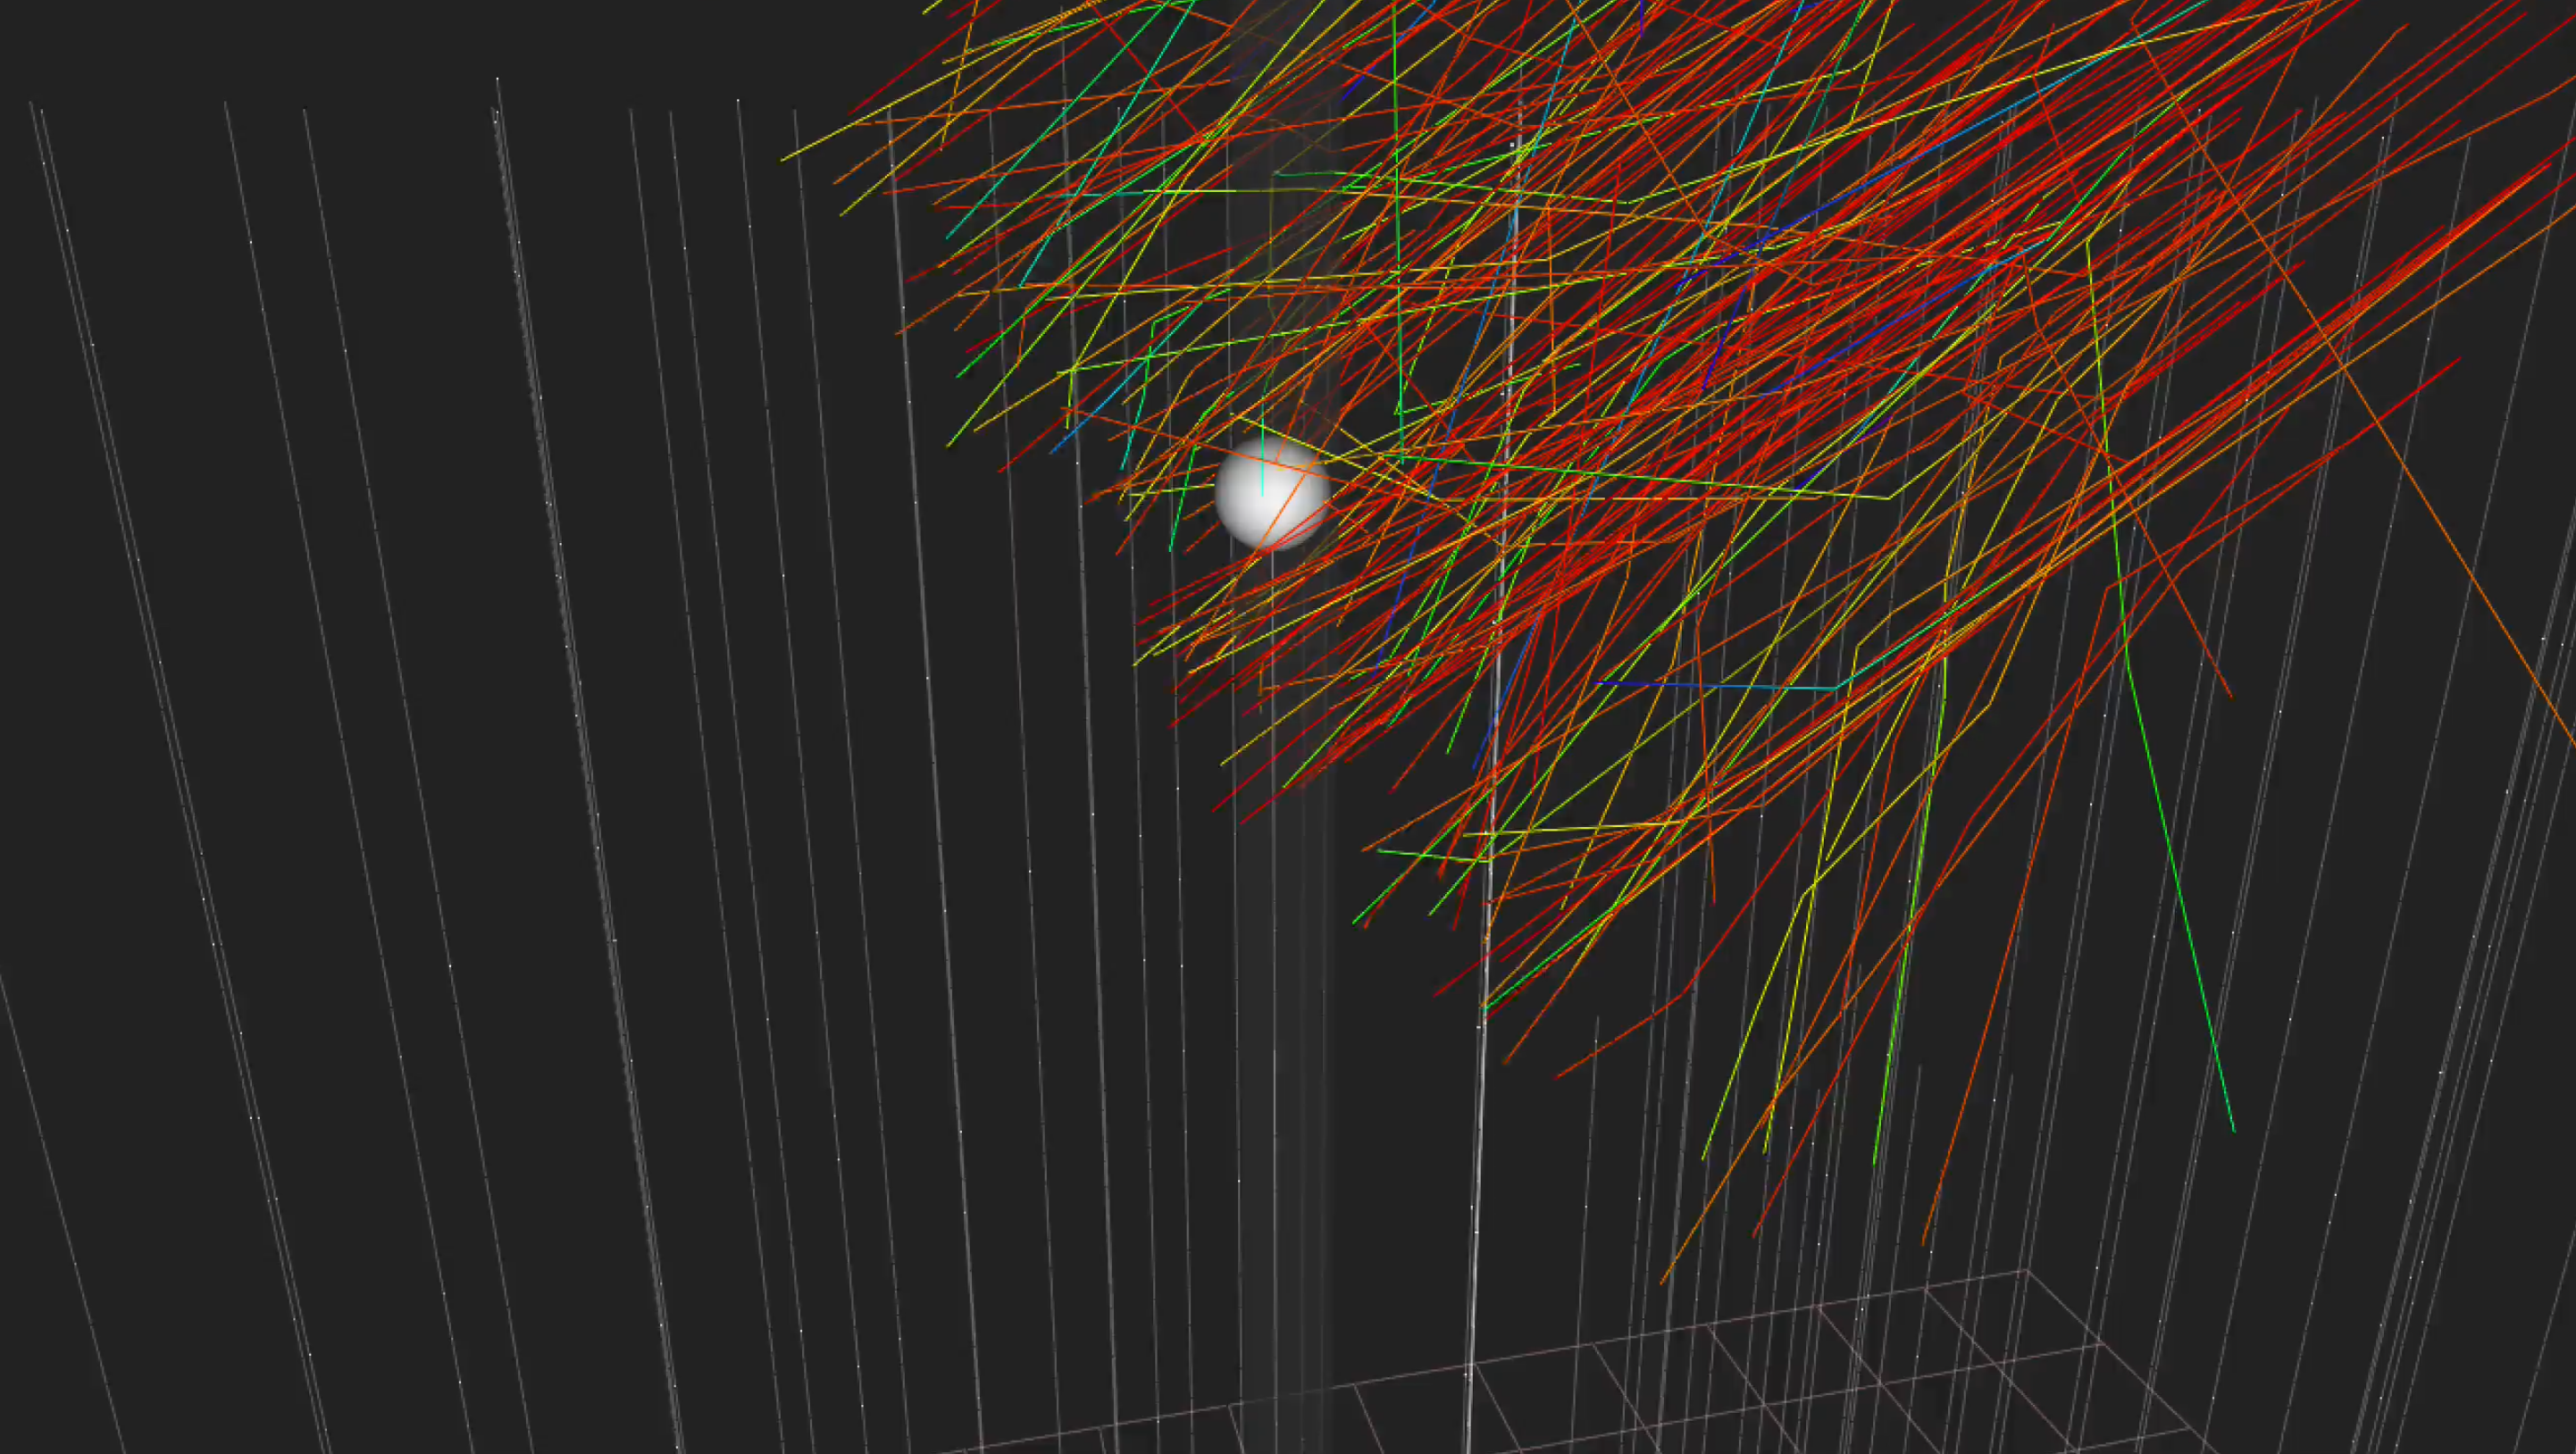
\includegraphics[height=3cm]{img/summerscenario-steamshovel}

  YouTube video of the simulation:

  \url{https://www.youtube.com/watch?v=M_QGNdGG9Ew}

  \end{center}
\end{frame}